
\documentclass[letterpaper,hide notes,xcolor={table,svgnames},pdftex]{beamer}
\def\showexamples{t}


%\usepackage[svgnames]{xcolor}

%% Demo talk
%\documentclass[letterpaper,notes=show]{beamer}

\usecolortheme{crane}%seahorse crane
\setbeamertemplate{navigation symbols}{}

\usetheme{MyPittsburgh}
%\usetheme{Frankfurt}

%\usepackage{tipa}

\usepackage{hyperref}
\usepackage{graphicx,xspace}
\usepackage[normalem]{ulem}

\newcommand\SF[1]{$\bigstar$\footnote{SF: #1}}

\usepackage{paratype}
\renewcommand*\familydefault{\sfdefault} %% Only if the base font of the document is to be sans serif
\usepackage[zerostyle=c]{newtxtt}
\usepackage[T1]{fontenc}

\newcounter{tmpnumSlide}
\newcounter{tmpnumNote}

\usepackage{xcolor}
\usepackage{tabu}
\definecolor{light-gray}{gray}{0.75}
\taburulecolor{light-gray}

% old question code
%\newcommand\question[1]{{$\bigstar$ \small \onlySlide{2}{#1}}}
% \newcommand\nquestion[1]{\ifdefined \presentationonly \textcircled{?} \fi \note{\par{\Large \textbf{?}} #1}}
% \newcommand\nanswer[1]{\note{\par{\Large \textbf{A}} #1}}


 \newcommand\mnote[1]{%
   \addtocounter{tmpnumSlide}{1}
   \ifdefined\showcues {~\tiny\fbox{\arabic{tmpnumSlide}}}\fi
   \note{\setlength{\parskip}{1ex}\addtocounter{tmpnumNote}{1}\textbf{\Large \arabic{tmpnumNote}:} {#1\par}}}

\newcommand\mmnote[1]{\note{\setlength{\parskip}{1ex}#1\par}}

%\newcommand\mnote[2][]{\ifdefined\handoutwithnotes {~\tiny\fbox{#1}}\fi
% \note{\setlength{\parskip}{1ex}\textbf{\Large #1:} #2\par}}

%\newcommand\mnote[2][]{{\tiny\fbox{#1}} \note{\setlength{\parskip}{1ex}\textbf{\Large #1:} #2\par}}

\newcommand\mquestion[2]{{~\color{red}\fbox{?}}\note{\setlength{\parskip}{1ex}\par{\Large \textbf{?}} #1} \note{\setlength{\parskip}{1ex}\par{\Large \textbf{A}} #2\par}\ifdefined \presentationonly \pause \fi}

\newcommand\blackboard[1]{%
\ifdefined   \showblackboard
  {#1}
  \else {\begin{center} \fbox{\colorbox{blue!30}{%
         \begin{minipage}{.95\linewidth}%
           \hspace{\stretch{1}} Some space intentionally left blank; done at the blackboard.%
         \end{minipage}}}\end{center}}%
         \fi%
}



%\newcommand\q{\tikz \node[thick,color=black,shape=circle]{?};}
%\newcommand\q{\ifdefined \presentationonly \textcircled{?} \fi}

\usepackage{listings}
\lstset{%
  keywordstyle=\bfseries,
  aboveskip=15pt,
  belowskip=15pt,
  captionpos=b,
  identifierstyle=\ttfamily,
  escapeinside={(*@}{@*)},
  stringstyle=\ttfamiliy,
  frame=lines,
  numbers=left, basicstyle=\scriptsize, numberstyle=\tiny, stepnumber=0, numbersep=2pt}

\usepackage{siunitx}
\newcommand\sius[1]{\num[group-separator = {,}]{#1}\si{\micro\second}}
\newcommand\sims[1]{\num[group-separator = {,}]{#1}\si{\milli\second}}
\newcommand\sins[1]{\num[group-separator = {,}]{#1}\si{\nano\second}}
\sisetup{group-separator = {,}, group-digits = true}

%% -------------------- tikz --------------------
\usepackage{tikz}
\usetikzlibrary{positioning}
\usetikzlibrary{arrows,backgrounds,automata,decorations.shapes,decorations.pathmorphing,decorations.markings,decorations.text}

\tikzstyle{place}=[circle,draw=blue!50,fill=blue!20,thick, inner sep=0pt,minimum size=6mm]
\tikzstyle{transition}=[rectangle,draw=black!50,fill=black!20,thick, inner sep=0pt,minimum size=4mm]

\tikzstyle{block}=[rectangle,draw=black, thick, inner sep=5pt]
\tikzstyle{bullet}=[circle,draw=black, fill=black, thin, inner sep=2pt]

\tikzstyle{pre}=[<-,shorten <=1pt,>=stealth',semithick]
\tikzstyle{post}=[->,shorten >=1pt,>=stealth',semithick]
\tikzstyle{bi}=[<->,shorten >=1pt,shorten <=1pt, >=stealth',semithick]

\tikzstyle{mut}=[-,>=stealth',semithick]

\tikzstyle{treereset}=[dashed,->, shorten >=1pt,>=stealth',thin]

\usepackage{ifmtarg}
\usepackage{xifthen}
\makeatletter
% new counter to now which frame it is within the sequence
\newcounter{multiframecounter}
% initialize buffer for previously used frame title
\gdef\lastframetitle{\textit{undefined}}
% new environment for a multi-frame
\newenvironment{multiframe}[1][]{%
\ifthenelse{\isempty{#1}}{%
% if no frame title was set via optional parameter,
% only increase sequence counter by 1
\addtocounter{multiframecounter}{1}%
}{%
% new frame title has been provided, thus
% reset sequence counter to 1 and buffer frame title for later use
\setcounter{multiframecounter}{1}%
\gdef\lastframetitle{#1}%
}%
% start conventional frame environment and
% automatically set frame title followed by sequence counter
\begin{frame}%
\frametitle{\lastframetitle~{\normalfont(\arabic{multiframecounter})}}%
}{%
\end{frame}%
}
\makeatother

\makeatletter
\newdimen\tu@tmpa%
\newdimen\ydiffl%
\newdimen\xdiffl%
\newcommand\ydiff[2]{%
    \coordinate (tmpnamea) at (#1);%
    \coordinate (tmpnameb) at (#2);%
    \pgfextracty{\tu@tmpa}{\pgfpointanchor{tmpnamea}{center}}%
    \pgfextracty{\ydiffl}{\pgfpointanchor{tmpnameb}{center}}%
    \advance\ydiffl by -\tu@tmpa%
}
\newcommand\xdiff[2]{%
    \coordinate (tmpnamea) at (#1);%
    \coordinate (tmpnameb) at (#2);%
    \pgfextractx{\tu@tmpa}{\pgfpointanchor{tmpnamea}{center}}%
    \pgfextractx{\xdiffl}{\pgfpointanchor{tmpnameb}{center}}%
    \advance\xdiffl by -\tu@tmpa%
}
\makeatother
\newcommand{\copyrightbox}[3][r]{%
\begin{tikzpicture}%
\node[inner sep=0pt,minimum size=2em](ciimage){#2};
\usefont{OT1}{phv}{n}{n}\fontsize{4}{4}\selectfont
\ydiff{ciimage.south}{ciimage.north}
\xdiff{ciimage.west}{ciimage.east}
\ifthenelse{\equal{#1}{r}}{%
\node[inner sep=0pt,right=1ex of ciimage.south east,anchor=north west,rotate=90]%
{\raggedleft\color{black!50}\parbox{\the\ydiffl}{\raggedright{}#3}};%
}{%
\ifthenelse{\equal{#1}{l}}{%
\node[inner sep=0pt,right=1ex of ciimage.south west,anchor=south west,rotate=90]%
{\raggedleft\color{black!50}\parbox{\the\ydiffl}{\raggedright{}#3}};%
}{%
\node[inner sep=0pt,below=1ex of ciimage.south west,anchor=north west]%
{\raggedleft\color{black!50}\parbox{\the\xdiffl}{\raggedright{}#3}};%
}
}
\end{tikzpicture}
}


%% --------------------

%\usepackage[excludeor]{everyhook}
%\PushPreHook{par}{\setbox0=\lastbox\llap{MUH}}\box0}

%\vspace*{\stretch{1}

%\setbox0=\lastbox \llap{\textbullet\enskip}\box0}

\setlength{\parskip}{\fill}

\newcommand\noskips{\setlength{\parskip}{1ex}}
\newcommand\doskips{\setlength{\parskip}{\fill}}

\newcommand\xx{\par\vspace*{\stretch{1}}\par}
\newcommand\xxs{\par\vspace*{2ex}\par}
\newcommand\tuple[1]{\langle #1 \rangle}
\newcommand\code[1]{{\sf \footnotesize #1}}
\newcommand\ex[1]{\uline{Example:} \ifdefined \presentationonly \pause \fi
  \ifdefined\showexamples#1\xspace\else{\uline{\hspace*{2cm}}}\fi}

\newcommand\ceil[1]{\lceil #1 \rceil}


\AtBeginSection[]
{
   \begin{frame}
       \frametitle{Outline}
       \tableofcontents[currentsection]
   \end{frame}
}



\pgfdeclarelayer{edgelayer}
\pgfdeclarelayer{nodelayer}
\pgfsetlayers{edgelayer,nodelayer,main}

\tikzstyle{none}=[inner sep=0pt]
\tikzstyle{rn}=[circle,fill=Red,draw=Black,line width=0.8 pt]
\tikzstyle{gn}=[circle,fill=Lime,draw=Black,line width=0.8 pt]
\tikzstyle{yn}=[circle,fill=Yellow,draw=Black,line width=0.8 pt]
\tikzstyle{empty}=[circle,fill=White,draw=Black]
\tikzstyle{bw} = [rectangle, draw, fill=blue!20, 
    text width=4em, text centered, rounded corners, minimum height=2em]
    
    \newcommand{\CcNote}[1]{% longname
	This work is licensed under the \textit{Creative Commons #1 3.0 License}.%
}
\newcommand{\CcImageBy}[1]{%
	\includegraphics[scale=#1]{creative_commons/cc_by_30.pdf}%
}
\newcommand{\CcImageSa}[1]{%
	\includegraphics[scale=#1]{creative_commons/cc_sa_30.pdf}%
}
\newcommand{\CcImageNc}[1]{%
	\includegraphics[scale=#1]{creative_commons/cc_nc_30.pdf}%
}
\newcommand{\CcGroupBySa}[2]{% zoom, gap
	\CcImageBy{#1}\hspace*{#2}\CcImageNc{#1}\hspace*{#2}\CcImageSa{#1}%
}
\newcommand{\CcLongnameByNcSa}{Attribution-NonCommercial-ShareAlike}


\newenvironment{changemargin}[1]{% 
  \begin{list}{}{% 
    \setlength{\topsep}{0pt}% 
    \setlength{\leftmargin}{#1}% 
    \setlength{\rightmargin}{1em}
    \setlength{\listparindent}{\parindent}% 
    \setlength{\itemindent}{\parindent}% 
    \setlength{\parsep}{\parskip}% 
  }% 
  \item[]}{\end{list}} 




\title{Lecture 2 --- Computer Basics; Intro to C++}

\author{J. Zarnett\\
\texttt{jzarnett@uwaterloo.ca}}
\institute{Department of Electrical and Computer Engineering \\
  University of Waterloo}
\date{\today}

\begin{document}

\begin{frame}
  \titlepage
  
  \begin{center}
  \small{Acknowledgments: W.D. Bishop}
  \end{center}
 \end{frame}
 
\part{Computer Basics}
\begin{frame}\partpage\end{frame}

\begin{frame}
\frametitle{von Neumann Computer Architecture}

\begin{center}
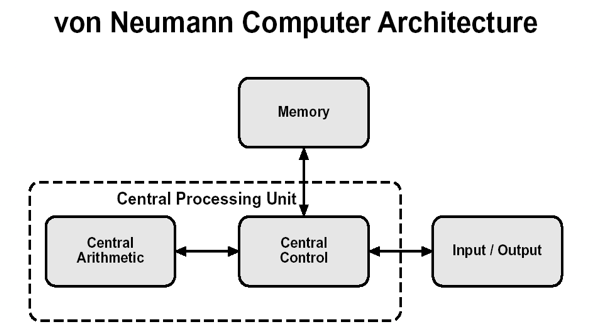
\includegraphics[width=0.75\textwidth]{images/vonNeumann.png}
\end{center}

\tiny{Source: J. von Neumann, First Draft of a Report on the EDVAC.  Technical Report W-6700RD-492, Moore School of Electrical Engineering, University of Pennsylvania, June 1945.}

\end{frame}

\begin{frame}
\frametitle{Central Processing Unit}

The CPU contains a central control unit and a central arithmetic unit.

CPU may also contain registers (high-speed storage locations) to store intermediate results and system state.

CPUs control computer systems using a sequence of instructions.\\
\quad Instructions manipulate data and control peripheral devices.

Intel Pentium IV processor is an example of a CPU.

\end{frame}

\begin{frame}
\frametitle{Central Control Unit}
Central control unit performs two functions:
\begin{enumerate}
\item Fetches instructions from memory
\item Performs instruction sequencing
\end{enumerate}

All information flow within the computer is directed by the central control unit.

\end{frame}

\begin{frame}
\frametitle{Central Control Unit}

Central arithmetic unit performs two functions:

\begin{enumerate}
\item Arithmetic operations (e.g., add, subtract, etc.)
\item Logic operations (e.g., bit-wise AND, bit-wise OR, etc.)
\end{enumerate}

Data is manipulated by the central arithmetic unit.

The central arithmetic unit is also sometimes called the \alert{arithmetic and logic unit (ALU)}.

\end{frame}

\begin{frame}
\frametitle{Memory Systems}

Memory systems use a linearly addressable array of cells to store binary information:
\begin{itemize}
	\item Each cell has a unique address
	\item Each cell stores a single binary digit (bit)
	\item  Cells are grouped to represent a larger range of possible values
\end{itemize}

\begin{center}
\begin{tabular}{l l l}
	\textbf{Grouping} & \textbf{Number of Bits} & \textbf{Number of Values Represented} \\ \hline
	Nybble & 4 bits & 16 values \\
	Byte   & 8 bits & 256 values \\
	Word   & $n$ bits & $2^{n}$ values \\
	Long Word & $2n$ bits & $2^{2n}$ values\\
\end{tabular}
\end{center}

\end{frame}

\begin{frame}
\frametitle{Memory Systems}

Memory systems can store both instructions and data.

Programs keep track of which memory cells contain instructions and which memory cells contain data.

\end{frame}

\begin{frame}
\frametitle{Input \& Output Systems}

\alert{Input / output (I/O)} systems allow the exchange of information between a computer system and its environment.

\begin{center}
\begin{tabular}{l l l l}
	\textbf{System Type} & \textbf{Source} & \textbf{Destination} & \textbf{Examples} \\ \hline
	Input & Environment & Computer & Keyboard, Mouse \\
	Output & Computer & Environment & Printer, Monitor\\
	I/O & Either & Either & Network Card, Modem\\
	\end{tabular}
\end{center}

\end{frame}

\begin{frame}
\frametitle{Basic Execution Cycle of a Computer}

Computers typically perform the following steps to execute a single instruction:
\begin{enumerate}
	\item Fetch the next instruction to be performed
	\item Decode the instruction
	\item Fetch operands (if necessary)
	\item Perform the operation
	\item Store the result (if necessary)
\end{enumerate}

Computers use a \alert{program counter} to store the address of the next instruction to be performed.

This counter is automatically updated by the computer as instructions are performed.


\end{frame}

\begin{frame}
\frametitle{Computer System}

Computer systems are comprised of hardware, software, and firmware.

\alert{Hardware} is a term for the physical components of a computer system. \\
\quad Examples include the CPU, network cards, etc. 

\alert{Software} is a term for the programs, procedures, and documentation associated with a computer system.\\
\quad Examples include MS-Word, MS-Excel, etc.

\alert{Firmware} is a term for programs stored within a read-only hardware device within a computer system.\\
\quad An example is the BIOS (Basic I/O System).


\end{frame}

\begin{frame}[fragile]
\frametitle{Computer Program}

A computer program is an instruction sequence to perform a particular task.

Programs can be created in machine language but this development process is very tedious.

As an example, the following machine language program adds two numbers on an Intel Pentium processor:
\begin{center}
{\small
\begin{verbatim}
	10100001 01101000 10111100 01000001 00000000
	00000011 00000101 01101100 10111100 01000001 00000000
	10100011 01110000 10111100 01000001 00000000
\end{verbatim}
}
\end{center}

Software developers use assemblers, interpreters, and compilers to build computer programs.

\end{frame}

\begin{frame}
\frametitle{Understanding Binary Quantities}
A sequence of 0s and 1s can have many meanings

Consider the quantity \texttt{1011001000100100}:

\begin{center}
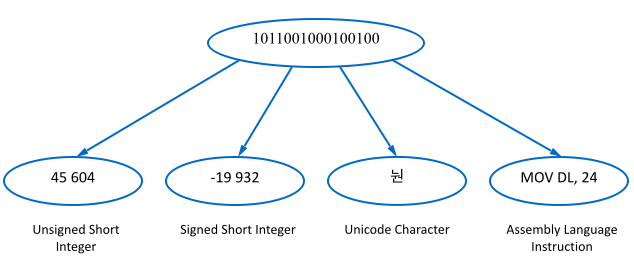
\includegraphics[width=0.85\textwidth]{images/binary.png}
\end{center}

Conclusion: \alert{Context is very important}.

\end{frame}

\begin{frame}
\frametitle{Assemblers}

\alert{Assembler}: a program to translate simple instructions named mnemonics from a human readable form to a machine readable form.

Assemblers translate assembly language into machine language.

Assembly language uses mnemonics to represent bit patterns.

Assembly language mnemonics (usually) have a 1:1 correspondence with machine language instructions.

\end{frame}

\begin{frame}
\frametitle{Interpreter}

An \alert{interpreter} is a program to translate a high-level description of a program into a machine readable form at execution time.

One statement in a high-level programming language may correspond with many machine language instructions.

Interpreters may be capable of performing code optimization at execution time.

\end{frame}

\begin{frame}
\frametitle{Compiler}

A \alert{compiler} is a program to translate a high-level description of a program into a machine readable form prior to execution.

One statement in a high-level programming language may correspond with many machine language instructions.

Compilers can perform code optimization at compile time.

Free compilers exist for all popular high-level programming languages including C, C++, Java, and C\#.

\end{frame}

\begin{frame}
\frametitle{Just-In-Time (JIT) Compilers}

A \alert{just-in-time compiler} is a special class of compiler.

Like interpreters, just-in-time compilers translate high-level descriptions of programs at execution time.

However, unlike interpreters, just-in-time compilers use a two stage compilation process.

\end{frame}

\begin{frame}
\frametitle{Just-In-Time (JIT) Compilers}
This allows code optimization at both compile and execution time.

Programs are first compiled into an intermediate language that is independent of the machine language of the computer.

At execution time, the intermediate language is translated to machine language by the JIT compiler.

\end{frame}

\begin{frame}
\frametitle{High-Level Programming Languages}

\alert{High-level programming languages} make it easier to develop, test, maintain, and reuse software.

Two programming paradigms are popular:
\begin{itemize}
	\item Structured Programming (SP):  A program is designed using a top-down approach based on the use of instruction sequences called functions
	\item Object-Oriented Programming (OOP):  A program is designed using a set of objects that encapsulate data and the functions performed on the data
\end{itemize}

Other programming paradigms exist but are rarely used.


\end{frame}


\begin{frame}
\frametitle{Syntax}

\alert{Syntax} refers to the way in which language constructs are written to form a computer program.

Forgetting a semicolon at the end of a line is a syntax error.

Missing a closing quote on a string is an example of a common syntax error.

Syntax errors prevent compilation.

Context-sensitive text editors can help reduce the frequency of syntax errors prior to compilation.

\end{frame}

\begin{frame}
\frametitle{Semantics}

\alert{Semantics} refers to the underlying meaning of a language construct.

Using the incorrect loop construct for a particular problem is an example of an error in semantics.

Errors in semantics do not prevent compilation but do result in a program behaving unexpectedly.

Errors in semantics can only be avoided by thoroughly understanding the programming language.

\end{frame}

\begin{frame}
\frametitle{Types of Software}

\alert{Application software} solves a problem or provides a service in a particular application domain.

Examples: word processors, spreadsheets, and engineering software.
\end{frame}

\begin{frame}
\frametitle{Types of Software}
\alert{System software} supports the development and use of application software.

Examples: operating systems, software development kits, and compilers.

\end{frame}


\begin{frame}
\frametitle{The Software Design Process}

\vspace{5em}

\begin{quote}
There are two ways of constructing a software design. One way is to make it so simple that there are obviously no deficiencies. And the other way is to make it so complicated that there are no obvious deficiencies.
\end{quote}
\hfill - C. A. R. Hoare


\end{frame}

\begin{frame}
\frametitle{The Software Design Process}


Software design is an iterative process.

The steps are:
\begin{enumerate}
	\item Define the problem
	\item Develop an algorithm to solve the problem
	\begin{itemize}
		\item Determine the sequence of steps required to solve a problem
		\item Several algorithms may exist to solve a specific problem
		\item Algorithm development may involve evaluating >1 option
	\end{itemize}
	\item Convert the algorithm to a specification in a suitable high-level programming language
	\item Debug the computer program
	\item Verify the operation of the computer program on a carefully chosen set of inputs
\end{enumerate}

\end{frame}

\begin{frame}
\frametitle{Software Documentation}

Software documentation describes the behaviour of software using text and/or graphics.

Documentation is an essential part of software development.

Well-documented software is easier to understand and maintain.

Often, three software documentation approaches are used:

\begin{itemize}
\item Pseudocode in the early stages of algorithm design
\item Unified Modeling Language (UML) in the latter stages of design
\item Source code comments during the construction of designs
\end{itemize}

\end{frame}

\part{Elements of a Program}
\begin{frame}\partpage\end{frame}

\begin{frame}
\frametitle{Elements of a Program}

At a very high level, a program consists of just data and instructions.

In memory, they look the same: a sequence of 1s and 0s.

We build a program by writing instructions to use \& manipulate data.

Thus, instructions are the building blocks of programming.

\end{frame}

\begin{frame}
\frametitle{Elements of a Program: Instructions}

Our programs will be built using the following elements:
\begin{itemize}
	\item Variable declarations define storage for data
	\item Assignment statements assign a value to variable
	\item Loop statements perform repetitive tasks
	\item Selection statements choose between 2+ paths of execution
	\item Function declarations define a reusable set of statements
	\item Function invocations use a function to perform a task
	\item Input statements retrieve data from a computing device
	\item Output statements send data to a computing device
\end{itemize}

As we go through the course, we'll learn about each of these.

\end{frame}

\begin{frame}
\frametitle{Elements of a Program: Instructions}

Each instruction has a specific format.\\
\quad The format is defined by the programming language standard.

Failure to follow the format may be a syntax or semantic error.

An instruction is built of one or more words or symbols.

\end{frame}

\begin{frame}
\frametitle{Keywords, Identifiers, and Literals}

\alert{Keywords} are language-defined reserved words.\\
	\quad Keywords denote language constructs.\\
	\quad Keywords may be reserved always or reserved in certain contexts.
	

\alert{Identifiers} are user-defined reserved words.\\
	\quad Identifiers denote classes, variables, functions, and constants.\\
	\quad Identifiers must start with a letter.\\
	\quad Identifiers are case-sensitive.\\
	\quad Keywords may not be used as identifiers.
	
	
\alert{Literals} are constant values that can be assigned to variables.\\
	\quad Literals are associated with a particular data type\\
	\quad The data type of a literal is determined by:\\
	\quad\quad its usage in the program and the way it is formatted.


\end{frame}

\begin{frame}
\frametitle{Keywords}

In any modern programming text editor, keywords will be highlighted.

This will help you spot them in the program, and also help you recognize that you cannot use one as an identifier name.

Don't attempt to memorize the list of keywords. If you practice programming, you will become familiar with the important ones.

\end{frame}

\begin{frame}
\frametitle{Program Structure}

All programs consist of many lines of code.

For a very simple program, this will all be in one file.

Complex programs will use multiple files \& folders of files...

\end{frame}

\begin{frame}
\frametitle{User Interface}
Programs almost always have a user interface: the part of the software that interacts with humans.

In this course, we'll work with Console Applications that interact with the user just via text on the screen and keyboard input.

Most of the pieces of software you are familiar with have \alert{Graphical User Interfaces (GUIs)} with pictures (icons) and buttons.

GUIs may look really neat, but they are complex and focus on them would be a barrier to learning the programming fundamentals.

\end{frame}


\part{Introduction to C++}
\begin{frame}\partpage\end{frame}

\begin{frame}
\frametitle{The C++ Programming Language}
\alert{C++} (``See Plus Plus'') is general purpose computing language.

It is based on the C programming language.

It is compiled, and can be imperative or object-oriented.

It is also a \alert{high level language}:\\
\quad\quad One keyword may equal many machine instructions.

\end{frame}


\begin{frame}
\frametitle{C++ Reserved Keywords}
{\scriptsize\tt
\vspace{-1.3em}
\begin{center}
\begin{tabular}{l l l l l}
alignas & alignof & and & and\_eq & asm \\ 
atomic\_cancel & atomic\_commit  & atomic\_noexcept & auto & bitand \\
bitor & bool & break & case & catch \\
char & char16\_t & char32\_t & class & compl \\ 
concept & const & constexpr & const\_cast & continue \\ 
decltype & default & delete & do & double \\ 
dynamic\_cast & else & enum & explicit & export \\
extern & false & float & for & friend \\ 
goto & if & inline & int & import \\ 
long & module & mutable & namespace & new \\ 
noexcept & not & not\_eq & nullptr & operator \\ 
or & or\_eq & private & protected & public \\
register & reinterpret\_cast & requires & return & short \\
signed & sizeof & static & static\_assert & static\_cast \\ 
struct & switch & synchronized & template & this \\ 
thread\_local & throw & true & try & typedef \\ 
typeid & typename & union & unsigned & using \\ 
virtual & void & volatile & wchar\_t & while \\
xor & xor\_eq & &\\
\end{tabular}
\end{center}
}
Don't try to memorize all of these; as we go through the course we will use some, but not all, of them.\\{\scriptsize Source: \url{http://en.cppreference.com/w/cpp/keyword}}
\end{frame}

\begin{frame}
\frametitle{C++ Contextual Keywords}

There are a few more keywords that are reserved in certain contexts.

You can use one as an identifier, but it's very bad practice:

{\small\tt
\begin{center}
\begin{tabular}{l l l l}
override & final & transaction\_safe & transaction\_safe\_dynamic\\
\end{tabular}
\end{center}
}
{\scriptsize Source: \url{http://en.cppreference.com/w/cpp/keyword}}
\end{frame}


\begin{frame}
\frametitle{C++ Programming}
To create and run a C++ program, the flow looks something like this:

\begin{enumerate}
	\item Write the program in an editor
	\item Compile the program
	\item Launch the program
	\item The program executes
\end{enumerate}

In the next lecture we'll create our very first C++ Program:\\
\quad Hello World.

\end{frame}


\end{document}

